%\documentclass[12pt]{article}

\questionheader{ex:s1.6}

%%%%%%%%%%%%%%%%%%%
%\subsection*{Derivatives, Velocity, Etc.}
%%%%%%%%%%%%%%%%%%%


%%%%%%%%%%%%%%%%%%
\subsection*{\Conceptual}
%%%%%%%%%%%%%%%%%%

%%%%%%%%%%%%%%%%%%%%%%%%%%%
\Instructions{Questions~\ref{prob_s1.0first} through \ref{prob_s1.0last} provide practice with curve parametrization. Being comfortable with the 
algebra and interpretation of these descriptions are essential ingredients 
in working effectively with parametrizations.}
%%%%%%%%%%%%%%%%%%%
\begin{question}\label{prob_s1.0first}
Consider the following time-parametrized curve:
\[\vr(t)=\left( \cos\left(\frac{\pi}{4}t\right)~,~(t-5)^2\right)\]

List the three points $(-1/\sqrt{2},0)$, $(1,25)$, and $(0,25)$ in chronological order.
\end{question}
\begin{hint}
Find the value of $t$ at which the three points occur on the curve.
\end{hint}
\begin{answer}
$(1,25)$, $(-1/\sqrt2,0)$, $(0,25)$.
\end{answer}
\begin{solution}
We can find the time at which the curve hits a given point by considering the two equations that arise from the two coordinates. For the $y$-coordinate to be 0, we must have $(t-5)^2=0$, i.e. $t=5$. So, the point $(-1/\sqrt{2},0)$ happens when $t=5$.

Similarly, for the $y$-coordinate to be $25$,  we need $(t-5)^2=25$, so $(t-5)=\pm 5$.
When $t=0$, the curve hits $(1, 25)$; when $t=10$, the curve hits $(0,25)$.

So, in order, the curve passes through the points $(1,25)$, $(-1/\sqrt2,0)$, and $(0,25)$.
\end{solution}
%%%%%%%%%%%%%%%%%%%

\begin{question}
At what points in the $xy$-plane does the curve $(\sin t, t^2)$ cross itself? What is the difference in $t$ between the first time the curve crosses through a point, and the last?
\end{question}
\begin{hint}
The curve ``crosses itself" when $(\sin t,t^2)$ gives the same coordinate for different values of $t$. When these crossings occur will depend on which crossing you're referring to, so your answers should all depend on $t$.
\end{hint}
\begin{answer}
The curve crosses itself at all points $(0,(\pi n)^2)$ where $n$ is an integer. It passes such a point twice, $2\pi n$ time units apart.
\end{answer}
\begin{solution}
The curve ``crosses itself" when the same coordinates occur for different values of $t$, say $t_1$ and $t_2$. So, we want to know when $\sin t_1=\sin t_2$ and also $t_1^2=t_2^2$. Since $t_1$ and $t_2$ should be different, the second equation tells us $t_2=-t_1$. Then the first equation tells us $\sin t_1=\sin t_2=\sin(-t_1)=-\sin t_1$. That is, $\sin t_1 = -\sin t_1$, so $\sin t_1=0$. That happens whenever $t_1=\pi n$ for an integer $n$.

So, the points at which the curve crosses itself are those points $(0,(\pi n)^2)$ where $n$ is an integer. It passes such a point at times $t=\pi n $ and $t=-\pi n$. So, the curve hits this point $2\pi n$ time units apart.
\end{solution}

%%%%%%%%%%%%%%%%%%%%%%%%%%%%%%%
\begin{question}
Find the specified parametrization of the first quadrant part
of the circle $x^2+y^2=a^2$.
\begin{enumerate}[(a)]
\item 
  In terms of the $y$ coordinate.
\item
  In terms of the angle between the tangent line and the 
  positive $x$-axis.
\item
  In terms of the arc length from $(0,a)$.
\end{enumerate}
\end{question}

\begin{hint} 
Draw sketches. Don't forget the range that the parameter runs over.
\end{hint}

\begin{answer} 
(a) $\vr(y)=\sqrt{a^2-y^2}\,\hi+ y\,\hj$, $0\le y\le a$

(b) $\big(x(\phi),y(\phi)\big)
       =\big(a\sin \phi ,-a\cos \phi \big)$,
   $\frac{\pi}{2}\le\phi\le\pi$

(c) $\big(x(s),y(s)\big)
    =\big(a\cos(\tfrac{\pi}{2}-\frac{s}{a}),
           a\sin(\tfrac{\pi}{2}-\tfrac{s}{a})\big)$,
   $0\le s\le\tfrac{\pi}{2}a$
\end{answer}

\begin{solution} 
(a) 
Since, on the specified part of the  circle, 
$x=\sqrt{a^2-y^2}$ and  $y$ runs from $0$ to $a$, 
the parametrization is
$\vr(y)=\sqrt{a^2-y^2}\,\hi+ y\,\hj$, $0\le y\le a$.

(b) Let $\theta$ be the angle between 
\begin{itemize}\itemsep1pt \parskip0pt \parsep0pt
\item the radius vector from the origin to the point 
$(a\cos\theta,a\sin\theta)$  on the circle and 
\item
the positive $x$-axis. 
\end{itemize}
The tangent line to the circle at $(a\cos\theta,a\sin\theta)$ 
is perpendicular to the radius vector and so makes angle $\phi=\frac{\pi}{2}+\theta$ with the positive $x$ axis.
(See the figure on the left below.)
As $\theta =\phi-\frac{\pi}{2}$, the desired parametrization is
\begin{equation*}
\big(x(\phi),y(\phi)\big)
=\big(a\cos(\phi-\tfrac{\pi}{2}),a\sin(\phi-\tfrac{\pi}{2})\big)
=\big(a\sin \phi ,-a\cos \phi \big),\ 
  \tfrac{\pi}{2}\le\phi\le\pi
\end{equation*}

\begin{center}
       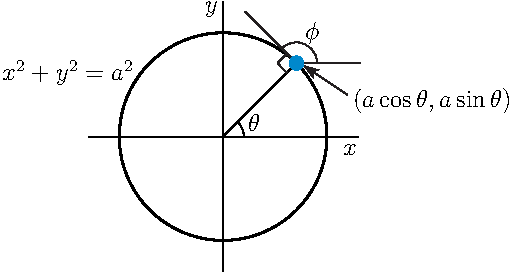
\includegraphics{parCirclePhi.pdf}\quad
       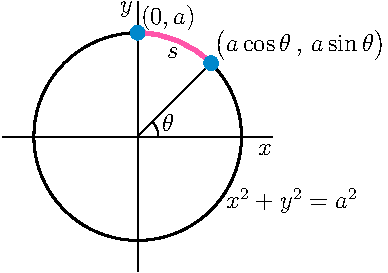
\includegraphics{parCircleS.pdf}
\end{center}


(c) Let $\theta$ be the angle between 
\begin{itemize}\itemsep1pt \parskip0pt \parsep0pt
\item the radius vector from the origin to the point 
$(a\cos\theta,a\sin\theta)$  on the circle and 
\item
the positive $x$-axis. 
\end{itemize} 
The arc from $(0,a)$ to $(a\cos\theta,a\sin\theta)$ 
subtends an angle $\frac{\pi}{2}-\theta$ and so
has length $s=a\big(\frac{\pi}{2}-\theta\big)$. (See the figure
on the right above.) Thus $\theta=\frac{\pi}{2}-\frac{s}{a}$
and the desired parametrization is
\begin{equation*}
\big(x(s),y(s)\big)
=\left(a\cos\left(\frac{\pi}{2}-\frac{s}{a}\right)\,,\,
           a\sin\left(\frac{\pi}{2}-\frac{s}{a}\right)\right)
,\ 0\le s\le\frac{\pi}{2}a
\end{equation*}
\end{solution}


%%%%%%%%%%%%%%%%%%%%%%%%%%%%%%%%%%%%%%
\begin{question}\label{prob_s1.1_cycloid}

\begin{center}
\begin{tikzpicture}
\YEaaxis{1}{13}{.5}{3}
\YExcoord{1}{1}
\YEycoord{1}{1}
\draw[thick] (1,2) node[red,vertex, label=above:{\textcolor{red}{$P$}}]{} arc (90:450:1cm);
\foreach \x in {0,1,2,3,4}{
	\MULTIPLY{\x}{.2}{\y}
	\SUBTRACT{1}{\y}{\o}
	\MULTIPLY{\x}{2.25}{\z}
	\MULTIPLY{\z}{57.3}{\zrad}
	\draw[red,opacity=\o] ({1+\z+sin(\zrad)},{1+cos(\zrad)}) node[vertex](P\x){};
	\draw[opacity=\o] ({1+\z},1) node[shape=circle, draw, minimum size=2cm]{}--(P\x);
		}
%\draw[thick, opacity=0.75] (1,2) node[red,vertex, label=above:{\textcolor{red}{$P$}}]{} arc (90:450:1cm);
\draw[red] plot[smooth,domain=0:13]({1+\x+sin(\x r)},{1+cos(\x r)});
\end{tikzpicture}
\end{center}

A circle of radius $a$ rolls along the $x$-axis in the positive direction, starting with its centre at $(a,a)$. In that position, we mark the topmost point on the circle $P$. As the circle moves, $P$ moves with it. Let $\theta$ be  the angle the circle has rolled--see the diagram below.
\begin{enumerate}[(a)]
\item Give the position of the centre of the circle as a function of $\theta$.
\item Give the position of $P$ a function of $\theta$.
\end{enumerate}
\begin{center}
\begin{tikzpicture}
\draw[thick] (0,0) node[shape=circle, minimum size=4cm, draw]{};
\draw (1.4,1.4)--(0,0)--(0,2);
\draw[red] (1.4,1.4) node[vertex, label= right:$P$](P){};
\draw[] (0,1) arc (90:45:1cm) node[midway, above]{$\theta$};
\draw[->] (0,2.5) arc(90:45:2.5cm);
\end{tikzpicture}
\end{center}

\end{question}
\begin{hint}
For part (b), find the position of $P$ relative to the centre of the circle. Then combine your answer with part (a).
\end{hint}
\begin{answer}
(a) $(a+a\theta,a)$\qquad
(b)$(a+a\theta+a\sin\theta,a+a\cos\theta)$
\end{answer}
\begin{solution}
Pretend that the circle is a spool of thread. As the 
           circle rolls it dispenses the thread along the ground.
           When the circle rolls $\theta$ radians it dispenses the
           arc length $\theta a$ of thread and the circle advances
           a distance $\theta a$. So centre of the circle has 
           moved $\theta a$ units to the right from its starting point, $x=a$. The centre of the circle always has $y$-coordinate $a$. So, after rolling $\theta$ radians, the centre of the circle is at position $\vc(\theta)=(a+a\theta,a)$.

Now, let's consider the position of $P$ on the circle, after the circle has rolled $\theta$ radians. 

\begin{center}
\begin{tikzpicture}
\draw[thick] (0,0) node[shape=circle, minimum size=8cm, draw]{};
\draw (2.8,2.8)--(0,0)--(0,4);
\draw[red] (2.8,2.8) node[vertex, label=above right:$P$](P){};
\draw[] (0,1) arc (90:45:1cm) node[midway, above]{$\theta$};
\draw[dashed] (P)--(0,2.8) node[midway, above]{$a\sin\theta$};
\draw[decorate, decoration={brace, amplitude=10pt}](-.25,0)--(-.25,2.8) node[midway,rotate=90,yshift=7.5mm]{$a\cos\theta$};
\draw[->] (0,5) arc(90:45:5cm);
\end{tikzpicture}
\end{center}
From the diagram, we see that $P$ is $a\cos \theta$ units above the centre of the circle, and $a\sin \theta$ units to the right of it. So, the position of $P$ is $(a+a\theta+a\sin\theta,a+a\cos\theta)$.

Remark: this type of curve is known as a \emph{cycloid}.
\end{solution}
%%%%%%%%%%%%%%%%%%%
\begin{question}\label{prob_s1.0last}
The curve $C$ is defined to be the intersection of the hyperboloid
\[x^2-\frac{1}{4}y^2+3z^2=1\]
and the plane
\[x+y+z=0.\]
When $y$ is very close to 0, and $z$ is negative, find an expression giving $z$ in terms of $y$.
\end{question}
\begin{hint}
We aren't concerned with $x$, so we can eliminate it by solving one equation for $x$ as a function
        of $y$ and $z$ and plugging the result into the other equation.
        \end{hint}
\begin{answer}
$z=-\frac12\sqrt{1-\frac{y^2}{2}}-\frac{y}{4}$
\end{answer}
\begin{solution}
We aren't concerned with $x$, so we can eliminate it by solving for it in one equation, and plugging that into the other. Since $C$ lies on the plane, $x=-y-z$, so:
\begin{align*}
1&=x^2-\frac{1}{4}y^2+3z^2=(-y-z)^2-\frac14y^2+3z^2\\
&=\frac{3}{4}y^2+4z^2+2yz
\intertext{Completing the square,}
1&=\frac{1}{2}y^2+\left(2z+\frac{y}{2}\right)^2\\
1-\frac{y^2}{2}&=\left(2z+\frac{y}{2}\right)^2
\intertext{Since $y$ is small, the left hand is close to $1$
         and the right hand side is close to $(2z)^2$.
         So $(2z^2)\approx 1$. Since $z$ is negative,
         $z\approx -\frac{1}{2}$ and  $2z+\frac{y}{2}<0$. Also, $1-\frac{y^2}{2}$ is positive, so it has a real square root.}
-\sqrt{1-\frac{y^2}{2}}&=2z+\frac{y}{2}\\
-\frac12\sqrt{1-\frac{y^2}{2}}-\frac{y}{4}&=z
\end{align*}

\end{solution}
%%%%%%%%%%%%%%%%%%%
\begin{question}
A particle traces out a curve in space, so that its position at time $t$ is \[\vr(t)=e^{-t}\,\hi+\frac{1}{t}\,\hj+(t-1)^2(t-3)^2\,\hk\] for $t > 0$. 

Let the positive $z$ axis point vertically upwards, as usual. When is the particle moving upwards, and when is it moving downwards? Is it moving faster at time $t=1$ or at time $t=3$?
\end{question}
\begin{hint}
To determine whether the particle is rising or falling, we only need to consider its $z$-coordinate. 
\end{hint}
\begin{answer}
The particle is moving upwards from $t=1$ to $t=2$, and from $t=3$ onwards.  The particle is moving downwards from $t=0$ to $t=1$, and from $t=2$ to $t=3$.

The particle is moving faster when $t=1$ than when $t=3$.
\end{answer}
\begin{solution}
To determine whether the particle is rising or falling, we only need to consider its $z$-coordinate: $z(t)=(t-1)^2(t-3)^2$. Its derivative with respect to time is $z'(t)=4(t-1)(t-2)(t-3)$. This is positive when $1<t<2$ and when $3<t$, so the particle is increasing on $(1,2) \cup (3,\infty)$ and decreasing on $(0,1) \cup (2,3)$.

If $\vr(t)$ is the position of the particle at time $t$, then its speed is $|\vr'(t)|$. We differentiate:
\[\vr'(t)=-e^{-t}\,\hi-\frac{1}{t^2}\,\hj+4(t-1)(t-2)(t-3)\hk\]
So, $\vr(1)=-\frac{1}{e}\,\hi-1\,\hj$ and $\vr(3)=-\frac{1}{e^3}\,\hi-\frac{1}{9}\,\hj$. The absolute value of every component of $\vr(1)$ is greater than or equal to that of the corresponding component of $\vr(3)$, so $|\vr(1)|>|\vr(3)|$. That is, the particle is moving more swiftly at $t=1$ than at $t=3$.

Note: We could also compute the sizes of both vectors directly: $|\vr'(1)|=\sqrt{\left(\frac{1}{e}\right)^2+(-1)^2}$, and $|\vr'(3)|=\sqrt{\left(\frac{1}{e^3}\right)^2+\left(-\frac{1}{9}\right)^2}$.
\end{solution}
%%%%%%%%%%%%%%%%%%%
\begin{question}
Below is the graph of the parametrized function $\vr(t)$. Let $s(t)$ be the arclength along the curve from $\vr(0)$ to $\vr(t)$.

\begin{center}
\begin{tikzpicture}
\draw[thick] plot[domain=-4.5:1]({4-\x*\x/4},\x);
\draw (4-1/16,-.5) node[vertex, label=right: $\vr(t+h)$](th){};
\draw (3,-2) node[vertex, label=right: $\vr(t)$](t){};
\draw (0,-4) node[vertex, label=below right: $\vr(0)$](zero){};
%\draw[|-|, red,yshift=10mm, xshift=-10mm] plot[domain=-4:-2]({4-\x*\x/4},\x);
%\draw[|-|, red,yshift=7.5mm, xshift=-7.5mm] plot[domain=-4:-.5]({4-\x*\x/4},\x);
%\draw[|-|, red,yshift=5mm, xshift=-5mm] plot[domain=-2:-.5]({4-\x*\x/4},\x);
%\draw[very thick, red, ->] (t)--(th);
\end{tikzpicture}
\end{center}
Indicate on the graph $s(t+h)-s(t)$ and $\vr(t+h)-\vr(t)$. Are the quantities scalars or vectors?

%Label $s(t)$, $s(t+h)$, $s(t+h)-s(t)$, and $\vr(t+h)-\vr(t)$. Which are scalars, and which are vectors?

%Lemma 1.1.3: draw a diagram, have students label $h$, $s(t+h)-s(t)$ etc.; which are constants, and which are vectors?
\end{question}
\begin{hint}
This is the setup from Lemma~\eref{CLP200}{lem:CVtanArclen} in the CLP-3 text. 
The two quantities you're labelling are related, but different.
\end{hint}
\begin{answer}

\begin{center}
\begin{tikzpicture}
\draw[thick] plot[domain=-4.5:1]({4-\x*\x/4},\x);
\draw (4-1/16,-.5) node[vertex, label=right: $\vr(t+h)$](th){};
\draw (3,-2) node[vertex, label=right: $\vr(t)$](t){};
\draw (0,-4) node[vertex, label=below right: $\vr(0)$](zero){};
%\draw[|-|, red,yshift=10mm, xshift=-10mm] plot[domain=-4:-2]({4-\x*\x/4},\x);
%\draw[|-|, red,yshift=7.5mm, xshift=-7.5mm] plot[domain=-4:-.5]({4-\x*\x/4},\x);
\draw[|-|, blue,yshift=-5mm, xshift=10mm] plot[domain=-2:-.5]({4-\x*\x/4},\x);
\draw[very thick, red, ->] (t)--(th);% node[midway, left]{$\vr(t+h)-\vr(t)$};
\end{tikzpicture}
\end{center}
The red vector is $\vr(t+h)-\vr(t)$. The arclength of the segment indicated by the blue line is the (scalar) $s(t+h)-s(t)$.

Remark: as $h$ approaches 0, the curve (if it's differentiable at $t$) starts to resemble a straight line, with the length of the vector $\vr(t+h)-\vr(t)$ approaching the scalar $s(t+h)-s(t)$. This step is crucial to understanding Lemma~\eref{CLP200}{lem:CVtanArclen} in the CLP-3 text. 
\end{answer}
\begin{solution}

\begin{center}
\begin{tikzpicture}
\draw[thick] plot[domain=-4.5:1]({4-\x*\x/4},\x);
\draw (4-1/16,-.5) node[vertex, label=right: $\vr(t+h)$](th){};
\draw (3,-2) node[vertex, label=right: $\vr(t)$](t){};
\draw (0,-4) node[vertex, label=below right: $\vr(0)$](zero){};
%\draw[|-|, red,yshift=10mm, xshift=-10mm] plot[domain=-4:-2]({4-\x*\x/4},\x);
%\draw[|-|, red,yshift=7.5mm, xshift=-7.5mm] plot[domain=-4:-.5]({4-\x*\x/4},\x);
\draw[|-|, blue,yshift=-5mm, xshift=10mm] plot[domain=-2:-.5]({4-\x*\x/4},\x);
\draw[very thick, red, ->] (t)--(th);% node[midway, left]{$\vr(t+h)-\vr(t)$};
\end{tikzpicture}
\end{center}
The red vector is $\vr(t+h)-\vr(t)$. The arclength of the segment indicated by the blue line is the (scalar) $s(t+h)-s(t)$.

Remark: as $h$ approaches 0, the curve (if it's differentiable at $t$) starts to resemble a straight line, with the length of the vector $\vr(t+h)-\vr(t)$ approaching the scalar $s(t+h)-s(t)$. This step is crucial to understanding Lemma~\eref{CLP200}{lem:CVtanArclen} in the CLP-3 text. 

\end{solution}
%%%%%%%%%%%%%%%%%%%
%%%%%%%%%%%%%%%%%%%
\begin{question}
What is the relationship between velocity and speed in a vector-valued function of time?
\end{question}
\begin{hint} See the note just before Example~\eref{CLP200}{eg:paramCircleTan}
in the CLP-3 text.
\end{hint}
\begin{answer}
Velocity is a vector-valued quantity, so it has both a magnitude and a direction. Speed is a scalar--the magnitude of the velocity. It does not include a direction.
\end{answer}
\begin{solution}
Velocity is a vector-valued quantity, so it has both a magnitude and a direction. Speed is a scalar--the magnitude of the velocity. It does not include a direction.\end{solution}
%%%%%%%%%%%%%%%%%%%

%%%%%%%%%%%%%%%%%%%
\begin{question}[M317 2005D] %1
Let $\vr(t)$ be a vector-valued function. Let $\vr'$, $\vr''$ , and $\vr'''$ 
denote $\diff{\vr}{t}$, $\difftwo{\vr}{t}$ and 
$\frac{\mathrm{d^3}\hfil\vr\hfil}{\mathrm{d}{t}^3}$, respectively.
Express
\begin{equation*}
\diff{\hfill}{t}\big[ (\vr \times \vr')\cdot\vr'' \big]
\end{equation*}
in terms of $\vr$, $\vr'$ , $\vr''$ , and $\vr'''$. 
Select the correct answer.
\begin{enumerate}[(a)]
\item\ \  $(\vr'\times\vr'' )\cdot\vr'''$
\item\ \  $(\vr'\times\vr'' )\cdot\vr + (\vr\times\vr' )\cdot\vr'''$
\item\ \  $(\vr\times\vr' )\cdot\vr'''$
\item\ \  $0$
\item\ \  None of the above.
\end{enumerate}
\end{question}

\begin{hint} 
To simplify your answer, remember: the cross product of $\va$ and $\vb$ is a vector orthogonal to both $\va$ and $\vb$; the cross product of a vector with itself is zero; and two orthogonal vectors have dot product 0.
\end{hint}

\begin{answer} 
(c)
\end{answer}

\begin{solution}
By the product rule
\begin{align*}
\diff{\hfill}{t}\big[ (\vr \times \vr')\cdot\vr'' \big]
&= (\vr' \times \vr')\cdot\vr''
  +(\vr \times \vr'')\cdot\vr''
  +(\vr \times \vr')\cdot\vr'''
\end{align*}
The first term vanishes because $\vr'\times\vr'=\vZero$.
The second term vanishes because $\vr \times \vr''$ is perpendicular to
$\vr''$. So
\begin{equation*}
\diff{\hfill}{t}\big[ (\vr \times \vr')\cdot\vr'' \big]
= (\vr \times \vr')\cdot\vr'''
\end{equation*}
which is (c).
\end{solution}
%%%%%%%%%%%%%%%%%%
\subsection*{\Procedural}
%%%%%%%%%%%%%%%%%%

%%%%%%%%%%%%%%%%%%%%%%%%%%%
\begin{question}[M317 2005D] %3
Find the speed of a particle with the given position function
\begin{equation*}
\vr(t) = 5 \sqrt{2}\,t\,\hi + e^{5t}\,\hj - e^{-5t}\,\hk
\end{equation*}
Select the correct answer:
\begin{enumerate}[(a)]
\item\ \ 
$|\vv(t)| = \big(e^{5t} + e^{-5t}\big)$
\item\ \ 
$|\vv(t)| = \sqrt{10 + 5e^{t} + 5e^{-t}}$
\item\ \ 
$|\vv(t)| = \sqrt{10 + e^{10t} + e^{-10t}}$
\item\ \ 
$|\vv(t)| = 5\big(e^{5t} + e^{-5t}\big)$
\item\ \ 
$|\vv(t)| = 5\big(e^t + e^{-t}\big)$
\end{enumerate}
\end{question}

\begin{hint} 
Just compute $|\vv(t)|$. Note that $\big(e^{at}+e^{-at}\big)^2 
=e^{2at} + 2 + e^{-2at}$.
\end{hint}

\begin{answer} 
(d)
\end{answer}

\begin{solution}
We have
\begin{equation*}
\vv(t) = \vr'(t) 
      = 5 \sqrt{2}\,\hi + 5e^{5t}\,\hj +5 e^{-5t}\,\hk
\end{equation*}
and hence
\begin{equation*}
|\vv(t)| = |\vr'(t)| 
         = 5 \big|\sqrt{2}\,\hi + e^{5t}\,\hj + e^{-5t}\,\hk\big|
         = 5\sqrt{2+ e^{10t}+ e^{-10t}}
\end{equation*}
Since $2+ e^{10t}+ e^{-10t} = \big(e^{5t}+e^{-5t}\big)^2$, that's (d).
\end{solution}


%%%%%%%%%%%%%%%%%%%%%%%%%%%%%%%%
\begin{question}
Find the velocity, speed and acceleration at time $t$ of
the particle whose position is $\vr(t)$. Describe the path of the particle.
Let $a>0$.
\begin{enumerate}[(a)]
\item
$\vr(t)= a \cos t\,\hi + a\sin t\,\hj + ct\,\hk$
\item
$\vr(t)= a \cos t\sin t\,\hi + a\sin^2 t\,\hj + a\cos t\,\hk$
\end{enumerate}
\end{question}

\begin{hint}
To figure out what the curves look like, first detemine what curve
$\big(x(t),y(t)\big)$ traces out. For part (b) this will be easier
if trig identities are first used to express $x(t)$ and $y(t)$ in terms of
$\sin(2t)$ and $\cos(2t)$.
\end{hint}

\begin{answer}
(a) 
\begin{align*}
\vv(t)&= -a \sin t\,\hi+a\cos t\,\hj+c\,\hk\\
\diff{s}{t}(t)&= \sqrt{a^2+c^2}\\
\va(t)&= -a \cos t\,\hi-a\sin t\,\hj
\end{align*}
The path is a helix with radius $a$ and with each turn having height $2\pi c$.

(b)
\begin{align*}
\vv(t)&= a \cos 2t\,\hi +a\sin 2t\,\hj-a\sin t\,\hk\\
\diff{s}{t}(t)&= a\sqrt{1+\sin^2t}\\
\va(t)&= -2a \sin 2t\,\hi +2a\cos 2t\,\hj-a\cos t\,\hk
\end{align*}
The $(x,y)$ coordinates go around a circle of radius $\frac{a}{2}$ and
centre $\big(0,\frac{a}{2}\big)$ counterclockwise. At the same time the $z$ coordinate oscillates over the interval between $1$ and $-1$ half as fast. In addition, the curve lies on 
the intersection of the cylinder $x^2+\big[y-\tfrac{a}{2}\big]^2=\tfrac{a^2}{4}$ and the sphere $x^2+y^2+z^2=a^2$. 
\end{answer}

\begin{solution}
(a) By definition,
\begin{align*}
\vr(t)&= a \cos t\,\hi+a\sin t\,\hj+ct\,\hk\\
\vv(t)=\vr'(t)&= -a \sin t\,\hi+a\cos t\,\hj+c\,\hk\\
\diff{s}{t}(t)=|\vv(t)|&= \sqrt{a^2+c^2}\\
\va(t)=\vr''(t)&= -a \cos t\,\hi-a\sin t\,\hj
\end{align*}
The $(x,y)= a(\cos t,\sin t)$ coordinates go 
     around a circle of radius $a$ and centre $(0,0)$ counterclockwise.
     One circle is completed for each increase of $t$ by $2\pi$.
     At the same time, the $z$ coordinate increases at a constant rate. 
     Each time the $(x,y)$ coordinates complete one circle, the $z$ 
     coordinate increases by $2 \pi c$.
The path is a helix with radius $a$ and with each turn having height $2\pi c$.

(b) By definition,
\begin{align*}
\vr(t)&= a \cos t\sin t\,\hi +a\sin^2 t\,\hj+a\cos t\,\hk\\
      &= \frac{a}{2} \sin 2t\,\hi+a\frac{1-\cos 2t}{2}\,\hj+a\cos t\,\hk\\
\vv(t)=\vr'(t)&= a \cos 2t\,\hi +a\sin 2t\,\hj-a\sin t\,\hk\\
\diff{s}{t}(t)=|\vv(t)|&= a\sqrt{1+\sin^2t}\\
\va(t)=\vr''(t)&= -2a \sin 2t\,\hi +2a\cos 2t\,\hj-a\cos t\,\hk
\end{align*}
Write
\begin{align*}
x(t)=\tfrac{a}{2} \sin 2t \qquad
y(t)=a\tfrac{1-\cos 2t}{2} \qquad
z(t)=a\cos t
\end{align*}
Then
\begin{align*}
x(t)^2+\big[y(t)-\tfrac{a}{2}\big]^2&=\tfrac{a^2}{4} \sin^2 2t + \tfrac{a^2}{4} \cos^2 2t 
                                     =\tfrac{a^2}{4} 
\end{align*}
Thus the $(x,y)$ coordinates go around a circle of radius $\frac{a}{2}$ and
centre $\big(0,\frac{a}{2}\big)$ counterclockwise. At the same time the $z$ coordinate oscillates over the interval between $1$ and $-1$ half as fast. In fact,
one can say more about the curve.
\begin{align*}
x(t)^2+y(t)^2&=\tfrac{a^2}{4} \sin^2 2t + \tfrac{a^2}{4}\big(1-\cos 2t\big)^2 \\
             &=\tfrac{a^2}{4} \sin^2 2t + \tfrac{a^2}{4} - \tfrac{a^2}{2}\cos 2t 
                 + \tfrac{a^2}{4} \cos^2 2t \\
             &= \tfrac{a^2}{2}  - \tfrac{a^2}{2} (1- 2\sin^2 t) \\
             &=  a^2\sin^2 t
\\
x(t)^2+y(t)^2+z(t)^2 &= a^2\sin^2 t + a^2\cos^2 t =a^2 
\end{align*}
So our curve lies on the intersection of the cylinder  
$x^2+\big[y-\tfrac{a}{2}\big]^2=\tfrac{a^2}{4}$ and the sphere $x^2+y^2+z^2=a^2$. 
(Don't worry if you didn't think of trying to evaluate $x(t)^2+y(t)^2+z(t)^2$.)
\end{solution}

%%%%%%%%%%%%%%%%%%%
\begin{question}[M317 2013D] %2

\begin{enumerate}[(a)]
\item
Let
\begin{equation*}
\vr(t) = \left(t^2 , 3, \tfrac{1}{3} t^3 \right) 
\end{equation*}
Find the unit tangent vector to this parametrized curve at $t = 1$, 
pointing in the direction of increasing $t$.
\item
Find the arc length of the curve from (a) between the points $(0, 3, 0)$ 
and $(1, 3, -\frac{1}{3})$.

\end{enumerate}
\end{question}

\begin{hint} 
Review Lemma \eref{CLP200}{lem:CVtanArclen} in the CLP-3 text.
The arc length should be positive.
\end{hint}

\begin{answer} 
(a) $\hat\vT(1) = \frac{(2,0,1)}{\sqrt{5}}$\qquad
(b) $\frac{1}{3}\big[5^{3/2}-8\big]$
\end{answer}

\begin{solution} (a)
Since $\vr'(t) = (2t,0,t^2)$, the specified unit tangent at $t=1$ is
\begin{equation*}
\hat\vT(1) = \frac{(2,0,1)}{\sqrt{5}}
\end{equation*}

\noindent (b)
We are to find the arc length between $\vr(0)$ and $\vr(-1)$. 
As $\diff{s}{t}=\sqrt{4t^2+t^4}$, the 
\begin{align*}
\text{arc length} &= \int_{-1}^0 \sqrt{4t^2+t^4}\ \dee{t}
\end{align*}
The integrand is even, so
\begin{align*}
\text{arc length} &= \int_0^1 \sqrt{4t^2+t^4}\ \dee{t}
=\int_0^1 t\sqrt{4+t^2}\ \dee{t}
=\Big[\tfrac{1}{3}{(4+t^2)}^{3/2}\Big]_0^1
=\tfrac{1}{3}\big[5^{3/2}-8\big]
\end{align*}

\end{solution}



%%%%%%%%%%%%%%%%%%%
\begin{question}\label{prob_s1.1:lemma113}
Using Lemma~\eref{CLP200}{lem:CVtanArclen} in the CLP-3 text, find the arclength of $\vr(t)=\left(t,\sqrt{\frac{3}{2}}t^2,t^3\right)$ from $t=0$ to $t=1$.
\end{question}
\begin{hint}
From Lemma~\eref{CLP200}{lem:CVtanArclen} in the CLP-3 text, 
we know the arclength from $t=0$ to $t=1$ will be
\[\int_{0}^1\left| \diff{\vr}{t}(t)\right|\dee t\]
The notation looks a little confusing at first, but we can break it down piece by piece: $\diff{\vr}{t}(t)$ is a vector, whose components are functions of $t$. If we take its magnitude, we'll get one big function of $t$. That function is what we integrate. Before integrating it, however, we should simplify as much as possible.
\end{hint}
\begin{answer}
2
\end{answer}
\begin{solution}
By Lemma~\eref{CLP200}{lem:CVtanArclen} in the CLP-3 text,  
the arclength of $\vr(t)$ from $t=0$ to $t=1$ is
$\int_{0}^1\left| \diff{\vr}{t}(t)\right|\dee t$. We'll calculate this in a few pieces to make the steps clearer.
\begin{align*}
\vr(t)&=\left(t,\sqrt{\frac{3}{2}}t^2,t^3\right)\\
\diff{\vr}{t}(t)&=\left(1,\sqrt{6}t,3t^2\right)\\
\left|\diff{\vr}{t}(t)\right|&=\sqrt{1^2+(\sqrt{6}t)^2+(3t^2)^2}=\sqrt{1+6t^2+9t^4}=\sqrt{(3t^2+1)^2}=3t^2+1\\
\int_{0}^1\left| \diff{\vr}{t}(t)\right|\dee t&=\int_0^1\left(3t^2+1 \right)\dee t=2
\end{align*}
\end{solution}
%%%%%%%%%%%%%%%%%%%
%%%%%%%%%%%%%%%%%%%

%%%%%%%%%%%%%%%%%%%%%%%%%%%%%%%%%%%%%%
\begin{question}
A particle's position at time $t$ is given by $\vr(t)=(t+\sin t, \cos t)$\footnote{The particle traces out a cycloid--see Question~\ref{prob_s1.1_cycloid}}. What is the magnitude of the acceleration of the particle at time $t$?
\end{question}
\begin{hint}
$\vr(t)$ is the position of the particle, so its acceleration is $\vr''(t)$.
\end{hint}
\begin{answer}
1
\end{answer}
\begin{solution}
Since $\vr(t)$ is the position of the particle,  its acceleration is $\vr''(t)$.
\begin{align*}
\vr(t)&=(t+\sin t, \cos t)\\
\vr'(t)&=(1+\cos t,-\sin t)\\
\vr''(t)&=(-\sin t,-\cos t)\\
|\vr''(t)|&=\sqrt{\sin^2t+\cos^2t}=1
\end{align*}
The magnitude of acceleration is constant, but its \emph{direction} is changing, since $\vr''(t)$ is a vector with changing direction.
\end{solution}



%%%%%%%%%%%%%%%%%%%%%%%%%%%
\begin{question}[M317 2011D] %2
A curve in $\bbbr^3$ is given by the vector equation 
$\vr(t) = \left(2t \cos t, 2t \sin t,\frac{t^3}{3}\right)$

\begin{enumerate}[(a)]
\item
Find the length of the curve between $t = 0$ and $t = 2$.

\item
Find the parametric equations of the tangent line to the curve at $t = \pi$.

\end{enumerate}
\end{question}

\begin{hint} 
Review \S\eref{CLP200}{sec lines 3d} and  Lemma \eref{CLP200}{lem:CVtanArclen} 
in the CLP-3 text.
\end{hint}

\begin{answer} 
(a) $\nicefrac{20}{3}$\qquad
(b) $x(t) = -2\pi -2t,\ 
     y(t) =  -2\pi t,\ 
     z(t) = \nicefrac{\pi^3}{3} + \pi^2 t$ 
\end{answer}

\begin{solution} (a) The speed is
\begin{align*}
\diff{s}{t}(t)
=\big|\vr'(t)\big| & = \left|\left(2\cos t - 2t\sin t\,,\,
                                  2\sin t + 2t \cos t\,,\,
                                  t^2\right)\right| \\
                  &=\sqrt{\big(2\cos t - 2t\sin t\big)^2
                         +\big(2\sin t + 2t \cos t\big)^2
                         +t^4} \\
                 &= \sqrt{4+ 4t^2 +t^4} \\
                 &= 2+t^2
\end{align*}
so the length of the curve is
\begin{align*}
\text{length }
&=\int_0^2 \diff{s}{t}\,\dee{t}
  =\int_0^2 (2+t^2)\,\dee{t}
  = \left[2t +\frac{t^3}{3}\right]_0^2
  =\frac{20}{3}
\end{align*}

\noindent (b)
A tangent vector to the curve at 
$\vr(\pi)=\big(-2\pi\,,\, 0\,,\, \nicefrac{\pi^3}{3}\big)$ is
\begin{equation*}
\vr'(\pi) = \left(2\cos\pi - 2\pi\sin\pi\,,\,
                                  2\sin\pi + 2\pi \cos\pi\,,\,
                                  \pi^2\right)
 = (-2\,,\,-2\pi\,,\,\pi^2)
\end{equation*}
So parametric equations for the tangent line at $\vr(\pi)$ are
\begin{align*}
x(t) &= -2\pi -2t \\
y(t) &=  -2\pi t \\
z(t) &= \nicefrac{\pi^3}{3} + \pi^2 t 
\end{align*}
\end{solution}
%%%%%%%%%%%%%%%%%%%%%%%%%%%%%%%

\begin{question}[M317 2010D]  %1
Let $\vr(t) = \big(3 \cos t, 3 \sin t, 4t\big)$ be the position vector 
of a particle as a function of time $t \ge 0$.
\begin{enumerate}[(a)]
\item
Find the velocity of the particle as a function of time $t$.
\item
Find the arclength of its path between $t = 1$ and $t = 2$.
\end{enumerate}
\end{question}

\begin{hint} 
Review Lemma \eref{CLP200}{lem:CVtanArclen} in the CLP-3 text.
\end{hint}

\begin{answer} 
(a) $\vr'(t) = \big(-3 \sin t, 3 \cos t, 4\big)$\qquad
(b) 5
\end{answer}

\begin{solution} (a) As $\vr(t) = \big(3 \cos t, 3 \sin t, 4t\big)$,
the velocity of the particle is
\begin{equation*}
\vr'(t) = \big(-3 \sin t, 3 \cos t, 4\big)
\end{equation*}

\noindent (b) As $\diff{s}{t}$, the rate of change of arc length per unit time,
is
\begin{equation*}
\diff{s}{t}(t) = |\vr'(t)| = \big|\big(-3 \sin t, 3 \cos t, 4\big)\big|
  =5
\end{equation*}
the arclength of its path between $t = 1$ and $t = 2$ is
\begin{equation*}
\int_1^2\dee{t}\ \diff{s}{t}(t) 
=\int_1^2\dee{t}\ 5
=5
\end{equation*}
\end{solution}


%%%%%%%%%%%%%%%%%%%%%%%%%%
\begin{question}[M317 2007A] %2
	Consider the curve
	\begin{equation*}
	\vr(t) = \frac{1}{3}\cos^3 t\,\hi +\frac{1}{3} \sin^3 t\,\hj + \sin^3 t\,\hk
	\end{equation*}
	\begin{enumerate}[(a)]
		\item
		Compute the arc length of the curve from $t = 0$ to $t = \frac{\pi}{2}$.
		\item
		Compute the arc length of the curve from $t = 0$ to $t = \pi$.
	\end{enumerate}
\end{question}

\begin{hint} 
	If you got the answer $0$ in part (b), you dropped some absolute value signs.
\end{hint}

\begin{answer} 
	(a) $\frac{1}{27}\big(10\sqrt{10}-1\big)$\qquad
	(b) $\frac{2}{27}\big(10\sqrt{10}-1\big)$
\end{answer}

\begin{solution} (a)
	As
	\begin{align*}
	\vr'(t) & = -\sin t\cos^2 t\,\hi + \sin^2 t\cos t\,\hi + 3\sin^2 t\cos t\,\hk
	= \sin t\cos t\big(-\cos t\,\hi +\sin t\,\hj +3\sin t\,\hk\big) \\
	\diff{s}{t}(t) & = |\sin t\cos t|\sqrt{\cos^2 t + \sin ^2 t + 9\sin^2 t}
	= |\sin t\cos t|\sqrt{1+ 9\sin^2 t}
	\end{align*}
	the arclength from $t = 0$ to $t = \frac{\pi}{2}$ is
	\begin{align*}
	\int_0^{\pi/2} \diff{s}{t}(t)\,\dee{t}
	&=\int_0^{\pi/2} \sin t\cos t \sqrt{1+ 9\sin^2 t}\,\dee{t} \\
	&=\frac{1}{18}\int_1^{10} \sqrt{u}\ \dee{u} \qquad
	\text{with } u = 1+ 9\sin^2 t,\ \dee{u}  = 18\sin t\cos t\,\dee{t}\\
	&=\frac{1}{18}\Big[\frac{2}{3}u^{3/2}\Big]_1^{10}\\
	&=\frac{1}{27}\big(10\sqrt{10}-1\big)
	\end{align*}
	
	(b) The arclength from $t = 0$ to $t = \pi$ is
	\begin{align*}
	\int_0^{\pi} \diff{s}{t}(t)\,\dee{t}
	&=\int_0^{\pi} |\sin t\cos t| \sqrt{1+ 9\sin^2 t}\,\dee{t} 
	\qquad\text{Don't forget the absolute value signs!}\\
	&=2\int_0^{\pi/2} |\sin t\cos t| \sqrt{1+ 9\sin^2 t}\,\dee{t} 
	= 2\int_0^{\pi/2} \sin t\cos t \sqrt{1+ 9\sin^2 t}\,\dee{t} 
	\end{align*}
	since the integrand is invariant under $t\rightarrow\pi-t$. So the arc length
	from $t = 0$ to $t = \pi$ is just twice the arc length from part (a), namely $\frac{2}{27}\big(10\sqrt{10}-1\big)$.
	
\end{solution}
%%%%%%%%%%%%%%%%%%%%%%%%%%%%%%%
\begin{question}[M317 2017D] %2
Let $\vr(t)=\big(\frac{1}{3}t^3,\frac{1}{2}t^2,\frac{1}{2}t\big)$,
$t\ge 0$. Compute $s(t$), the arclength of the curve at time
$t$.
\end{question}

%\begin{hint} 
%\end{hint}

\begin{answer} 
$s(t)=\frac{t^3}{3} +\frac{t}{2}$
\end{answer}

\begin{solution} 
Since
\begin{align*}
\vr(t)&= \frac{t^3}{3}\,\hi + \frac{t^2}{2}\,\hj +  \frac{t}{2}\,\hk\\
\vr'(t)&= t^2\,\hi + t\,\hj + \frac{1}{2}\,\hk \\
\diff{s}{t}(t)=|\vr'(t)|&=\sqrt{t^4+t^2+\frac{1}{4}}
=\sqrt{\Big(t^2+\frac{1}{2}\Big)^2}=t^2+\frac{1}{2}
\end{align*}
the length of the curve is
\begin{align*}
s(t)=\int_0^t \diff{s}{t}(u)\,\dee{u}
=\int_0^t \Big(u^2+\frac{1}{2}\Big)\,\dee{u}
=\frac{t^3}{3} +\frac{t}{2}
\end{align*}
\end{solution}


%%%%%%%%%%%%%%%%%%%%%%%%%%%%%%%
\begin{question}[M317 2011A] %3
Find the arc length of the curve 
$\vr(t) = \big(t^m\,,\, t^m\,,\, t^{3m/2}\big)$ for $0 \le a \le t \le b$, 
and where $m > 0$.
Express your result in terms of $m$, $a$, and $b$. 
\end{question}

\begin{hint} 
The integral you get can be evaluated with
a simple substitution. You may want to factor the integrand first.
\end{hint}

\begin{answer} 
$\frac{8}{27}\Big[\Big(2 + \frac{9}{4}b^m\Big)^{3/2}
                   -\Big(2 + \frac{9}{4}a^m\Big)^{3/2}\Big]$
\end{answer}

\begin{solution} 
Since
\begin{align*}
\vr(t) & = t^m\,\hi + t^m\,\hj + t^{3m/2}\,\hk \\
\vr'(t) &= mt^{m-1}\,\hi + mt^{m-1}\,\hj +\frac{3m}{2}t^{3m/2-1}\,\hk \\
\diff{s}{t} = |\vr'(t)| & = \sqrt{ 2m^2 t^{2m-2} +\frac{9m^2}{4} t^{3m-2} } 
= mt^{m-1}\sqrt{2 + \frac{9}{4}t^m }
\end{align*}
the arc length is
\begin{align*}
\int_a^b \diff{s}{t}(t)\,\dee{t}
&=\int_a^b mt^{m-1}\sqrt{2 + \frac{9}{4}t^m }\ \dee{t} \\
&=\frac{4}{9}\int_{2 + \frac{9}{4}a^m}^{2 + \frac{9}{4}b^m}\sqrt{u}\,\dee{u}
\qquad\text{with } u = 2 + \frac{9}{4}t^m,\ \dee{u} = \frac{9m}{4}t^{m-1}\\
&=\frac{4}{9}\Big[\frac{2}{3}u^{3/2}\Big]_{2 + \frac{9}{4}a^m}
                                         ^{2 + \frac{9}{4}b^m} \\
&=\frac{8}{27}\Big[\Big(2 + \frac{9}{4}b^m\Big)^{3/2}
                   -\Big(2 + \frac{9}{4}a^m\Big)^{3/2}\Big]
\end{align*} 
\end{solution}




%%%%%%%%%%%%%%%%%%%
\begin{question}
If a particle has constant mass $m$, position $\vr$, and is moving with velocity $\vv$, then its angular momentum is $\vL=m(\vr\times\vv)$. 

For a particle with mass $m=1$ and position function $\vr=(\sin t, \cos t, t)$, find $\left|\diff{\vL}{t} \right|$.

\end{question}
\begin{hint} 
Given the position of a particle, you can find its velocity.
\end{hint}
\begin{answer}
$|t|$
\end{answer}
\begin{solution}
Given the position of the particle, we can find its velocity:
\[\vv(t)=\vr'(t)=(\cos t, -\sin t , 1)\]
Applying the given formula,
\[\vL(t)=\vr \times \vv=(\sin t , \cos t , t) \times (\cos t, -\sin t , 1).\]
\begin{description}
\item[\textbf{Solution 1:}]
We can first compute the cross product, then differentiate:
\begin{align*}
\vL(t)& = (\cos t + t\sin t)\hi + (t\cos t - \sin t)\hj-\hk\\
\vL'(t)&=t\cos t\,\hi -t\sin t\, \hj\\
|\vL'(t)|&=\sqrt{t^2(\sin^2 t + \cos^2 t)}=\sqrt{t^2}=|t|
\end{align*}
\item[\textbf{Solution 2:}]
Using the product rule:
\begin{align*}
\vL'(t)&=\vr'(t)\times \vv(t) + \vr(t) \times \vv'(t)\\
&=\underbrace{\vr'(t)\times \vr'(t)}_{0} + \vr(t) \times \vv'(t)\\
&= (\sin t ,\cos t,t)\times(-\sin t , -\cos t, 0)\\
&=t\cos t\,\hi-t\sin t\,\hj\\
|\vL'(t)|&=\sqrt{t^2\cos^2 t + t^2\sin t^2  }=|t|
\end{align*}
\end{description}
\end{solution}

%%%%%%%%%%%%%%%%%%%%%%%%%%%%%%%%
\begin{question}[M200 2002A] %1
 Consider the space curve $\Ga$ whose vector equation is
\begin{equation*}
\vr(t)=t\sin(\pi t)\,\hi+t\cos(\pi t)\,\hj +t^2\hk\,\qquad 0\le t<\infty
\end{equation*}
This curve starts from the origin and eventually reaches the ellipsoid
$E$ whose equation is $2x^2+2y^2+z^2=24$.
\begin{enumerate}[(a)]
\item
Determine the coordinates of the point $P$ where $\Ga$ intersects $E$.

\item 
Find the tangent vector of $\Ga$ at the point $P$.

\item 
Does $\Ga$ intersect $E$ at right angles? Why or why not?
\end{enumerate}
\end{question}

%\begin{hint}
%\end{hint}

\begin{answer}
(a) $\vr(2)=2\hj+4\hk$\qquad
(b) any nonzero multiple of $\vr'(2)=2\pi\,\hi+\hj+4\,\hk$

(c) $\Ga$ and $E$ do not intersect at right angles.
\end{answer}

\begin{solution}
(a) The curve intersects $E$ when
\begin{equation*}
2\big(t\sin(\pi t)\big)^2+2\big(t\cos(\pi t)\big)^2 +\big(t^2\big)^2=24
\iff 2t^2+t^4=24
\iff (t^2-4)(t^2+6)=0
\end{equation*}
Since we need $t>0$, the desired time is $t=2$ and the corresponding point
is $\vr(2)=2\,\hj+4\,\hk$.

(b) Since
\begin{equation*}
\vr'(t)=\big[\sin(\pi t)+\pi t\cos(\pi t)\big]\hi
    +\big[\cos(\pi t)-\pi t\sin(\pi t)\big]\hj + 2t\hk
\end{equation*}
a tangent vector to $\Ga$ at $P$ is any nonzero multiple of
\begin{equation*}
\vr'(2)=2\pi\,\hi+\hj+4\,\hk
\end{equation*}

(c) A normal vector to $E$ at $P$ is
\begin{equation*}
\vnabla(2x^2+2y^2+z^2)\big|_{(0,2,4)}= \llt 4x,4y,2z\rgt\big|_{(0,2,4)}
=\llt 0,8,8\rgt
\end{equation*}
Since $\vr'(2)$ and $\llt 0,8,8\rgt$ are not parallel, $\Ga$ and $E$
do not intersect at right angles.
\end{solution}

%%%%%%%%%%%%%%%%%%%%%%%%%%%%%%%%%%%%%%%%%
\begin{question} [M200 2001A] % 6
Suppose a particle in 3-dimensional space travels with
position vector $\vr(t)$, which satisfies $\vr''(t)=-\vr(t)$. Show
that the ``energy'' $|\vr(t)|^2+|\vr'(t)|^2$ is constant (that is,
independent of $t$).
\end{question}

%\begin{hint}
%
%\end{hint}

\begin{answer}
$\diff{}{t}\big[|\vr(t)|^2+|\vr'(t)|^2\big]=0$
\end{answer}

\begin{solution}
\begin{align*}
\diff{}{t}\big[|\vr(t)|^2+|\vr'(t)|^2\big]
&=\diff{}{t}\big[\vr(t)\cdot\vr(t)+\vr'(t)\cdot\vr'(t)\big]\\
&=2\vr(t)\cdot\vr'(t)+2\vr'(t)\cdot\vr''(t)\\
&=2\vr'(t)\cdot\big[\vr(t)+\vr''(t)\big]\\
&=0\qquad \text{ since $\vr''(t)=-\vr(t)$ }
\end{align*}
Since $\diff{}{t}\big[|\vr(t)|^2+|\vr'(t)|^2\big]=0$ for all
$t$, $|\vr(t)|^2+|\vr'(t)|^2$ is independent of $t$.
\end{solution}




%%%%%%%%%%%%%%%%%
\subsection*{\Application}
%%%%%%%%%%%%%%%%%


%%%%%%%%%%%%%%%%%%%%%%%%%%%%
\begin{question}[M317 2000A] %1
 A particle moves along the curve $\cC$ of intersection of
the surfaces $z^2=12y$ and $18x=yz$ in the upward direction. When the particle
is at $(1,3,6)$ its velocity $\vv$ and acceleration $\va$ are given by
$$
\vv =6\,\hi+12\,\hj+12\,\hk\qquad
\va = 27\,\hi+30\,\hj+6\,\hk
$$
\begin{enumerate}[(a)]
\item
 Write a vector parametric equation for $\cC$ using 
$u=\frac{z}{6}$ as a parameter.
\item
 Find the length of $\cC$ from $(0,0,0)$ to $(1,3,6)$.
\item
 If $u=u(t)$ is the parameter value for the particle's position
at time $t$, find $\diff{u}{t}$ when the particle is at $(1,3,6)$.
\item
 Find $\difftwo{u}{t}$ when the particle is at $(1,3,6)$.
\end{enumerate}
\end{question}

\begin{hint} 
If $\vr(u)$ is the parametrization of $\cC$ by $u$, then
the position of the particle at time $t$ is $\vR(t) = \vr\big(u(t)\big)$.
\end{hint}

\begin{answer} 
(a)  $\vr(u)=u^3\,\hi+3u^2\,\hj+6u\,\hk$\qquad
(b)  $7$\qquad
(c)  $2$\qquad
(d)  $1$
\end{answer}

\begin{solution}
(a) 
Since $z=6u$, $y=\frac{z^2}{12}=3u^2$ and $x=\frac{yz}{18}=u^3$,
\begin{align*}
\vr(u)&=u^3\,\hi+3u^2\,\hj+6u\,\hk\cr
\end{align*}
(b)
\begin{align*}
\vr'(u)&=3u^2\,\hi+6u\,\hj+6\,\hk\cr
\vr''(u)&=6u\,\hi+6\,\hj\cr
\diff{s}{u}(u)=|\vr'(u)|
&=\sqrt{9u^4+36u^2+36}=3\big(u^2+2\big)\cr
%\diff{s}{u}(1)&=9
\end{align*}


$$
\int_\cC \ ds
=\int_0^1 \diff{s}{u}\ \dee{u}
=\int_0^1 3\big(u^2+2\big)\ \dee{u}
=\big[u^3+6u\big]_0^1
=7
$$

(c) Denote by $\vR(t)$ the position of the particle at time $t$.
Then
$$
\vR(t)=\vr\big(u(t)\big)\implies
\vR'(t)=\vr'\big(u(t)\big)\diff{u}{t}
$$
In particular, if the particle is at $(1,3,6)$ at time $t_1$, then $u(t_1)=1$
and
$$
6\,\hi+12\,\hj+12\,\hk=\vR'(t_1)=\vr'(1)\diff{u}{t}(t_1)
=\big(3\,\hi+6\,\hj+6\,\hk\big)\diff{u}{t}(t_1)
$$
which implies that $\diff{u}{t}(t_1)=2$.

(d) By the product and chain rules,
$$
\vR'(t)=\vr'\big(u(t)\big)\diff{u}{t}\implies
\vR''(t)=\vr''\big(u(t)\big)\Big(\diff{u}{t}\Big)^2
+\vr'\big(u(t)\big)\difftwo{u}{t}
$$
In particular,
\begin{align*}
27\,\hi+30\,\hj+6\,\hk
&=\vR''(t_1)=\vr''(1)\Big(\diff{u}{t}(t_1)\Big)^2
+\vr'\big(1\big)\difftwo{u}{t}(t_1) \\
&=\big(6\,\hi+6\,\hj\big)2^2+\big(3\,\hi+6\,\hj+6\,\hk\big)\difftwo{u}{t}(t_1)
\end{align*}
Simplifying
$$
3\,\hi+6\,\hj+6\,\hk
=\big(3\,\hi+6\,\hj+6\,\hk\big)\difftwo{u}{t}(t_1)
\implies \difftwo{u}{t}(t_1)=1
$$
\end{solution}


%%%%%%%%%%%%%%%%%%%%%%%%%%%
\begin{question}[M317 2008A] %2
A particle of mass $m = 1$ has position $\vr_0 = \frac{1}{2}\,\hk$ 
and velocity $\vv_0 =\frac{\pi^2}{2}\,\hi$ at time $0$.
It moves under a force
\begin{equation*}
\vF(t) = -3t\,\hi + \sin t\,\hj + 2e^{2t}\,\hk.
\end{equation*}
\begin{enumerate}[(a)]
\item
Determine the position $\vr(t)$ of the particle depending on $t$.
\item
At what time after time $t = 0$ does the particle cross the plane 
$x = 0$ for the first time?
\item
What is the velocity of the particle when it crosses the plane $x = 0$ 
in part (b)?
\end{enumerate}
\end{question}

\begin{hint} 
By Newton's law, $\vF=m\va$.
\end{hint}

\begin{answer} 
(a) $\vr(t) = \big(\frac{\pi^2 t}{2}-\frac{t^3}{2}\big)\,\hi + 
              (t- \sin t)\,\hj + \left(\frac{1}{2}e^{2t}-t\right)\,\hk$ \qquad
(b) $t=\pi$ 

(c) $-\pi^2\,\hi +2\,\hj + \big(e^{2\pi}-1\big)\,\hk$
\end{answer}

\begin{solution} (a)
According to Newton,
\begin{equation*}
m\vr''(t) = \vF(t)\qquad\text{so that}\qquad
\vr''(t) = -3t\,\hi + \sin t\,\hj + 2e^{2t}\,\hk
\end{equation*}
Integrating once gives
\begin{align*}
\vr'(t) = -3\frac{t^2}{2}\,\hi - \cos t\,\hj + e^{2t}\,\hk +\vc
\end{align*}
for some constant vector $\vc$. We are told that $\vr'(0)=\vv_0
=\frac{\pi^2}{2}\,\hi$. This forces $\vc=\frac{\pi^2}{2}\,\hi+\hj-\hk$
so that
\begin{align*}
\vr'(t) = \left(\frac{\pi^2}{2}-\frac{3t^2}{2}\right)\,\hi +(1- \cos t)\,\hj + \big(e^{2t}-1\big)\,\hk 
\end{align*}
Integrating a second time gives
\begin{align*}
\vr(t) = \left(\frac{\pi^2 t}{2}-\frac{t^3}{2}\right)\,\hi +(t- \sin t)\,\hj 
 + \left(\frac{1}{2}e^{2t}-t\right)\,\hk  + \vc
\end{align*}
for some (other) constant vector $\vc$.  We are told that $\vr(0)=\vr_0
=\frac{1}{2}\,\hk$. This forces $\vc=\vZero$
so that
\begin{align*}
\vr(t) = \left(\frac{\pi^2 t}{2}-\frac{t^3}{2}\right)\,\hi +(t- \sin t)\,\hj 
 + \left(\frac{1}{2}e^{2t}-t\right)\,\hk 
\end{align*}

(b) The particle is in the plane $x=0$ when
\begin{align*}
0=\left(\frac{\pi^2 t}{2}-\frac{t^3}{2}\right)
 =\frac{t}{2}(\pi^2-t^2) 
\iff t=0, \pm\pi
\end{align*}
So the desired time is $t=\pi$.

(c) At time $t=\pi$, the velocity is
\begin{align*}
\vr'(\pi) 
&= \left(\frac{\pi^2}{2}-\frac{3\pi^2}{2}\right)\,\hi +(1- \cos\pi)\,\hj +                 \big(e^{2\pi}-1\big)\,\hk \\
&= -\pi^2\,\hi +2\,\hj + \big(e^{2\pi}-1\big)\,\hk
\end{align*}

\end{solution}
%%%%%%%%%%%%%%%%%%%%%%%%%%%%
\begin{question}[M317 1999A] %1
 Let $C$ be the curve of intersection of
the surfaces $y=x^2$ and $z=\frac{2}{3}x^3$.
A particle moves along $C$ with constant speed such that $\diff{x}{t}>0$.
The particle is at $(0,0,0)$ at time $t=0$ and is at $(3,9,18)$ at time
$t=\frac{7}{2}$.
\begin{enumerate}[(a)]
\item
Find the length of the part of $C$ between $(0,0,0)$ and $(3,9,18)$.
\item
Find the constant speed of the particle.
\item
Find the velocity of the particle when it is at $\big(1,1,\frac{2}{3}\big)$.
\item
Find the acceleration of the particle when it is at $\big(1,1,\frac{2}{3}\big)$.
\end{enumerate}
\end{question}

\begin{hint} 
Denote by $\vr(x)$ the parametrization of $C$ by $x$. If the $x$--coordinate
of the particle at time $t$ is $x(t)$, then the position of the particle at time $t$ is $\vR(t)=\vr\big(x(t)\big)$. Also, though the particle is moving at a constant speed, it doesn't necessarily have a constant value of $\diff{\vx}{t}$.
\end{hint}

\begin{answer} 
(a) $21$\qquad
(b) $6$\qquad
(c) $2\hi+4\,\hj+4\,\hk$\qquad
(d) $-\frac{8}{3}\big(2\hi+\,\hj-2\,\hk\big)$
\end{answer}

\begin{solution}
(a) Parametrize $C$ by $x$. Since $y=x^2$ and $z=\frac{2}{3}x^3$,
\begin{align*}
\vr(x)&=x\,\hi+x^2\,\hj+\frac{2}{3}x^3\,\hk\cr
\vr'(x)&=\hi+2x\,\hj+2x^2\,\hk\cr
\vr''(x)&=2\,\hj+4x\,\hk\cr
\diff{s}{x}
&=|\vr'(x)|
=\sqrt{1+4x^2+4x^4}=1+2x^2\cr
\end{align*}
and
$$
\int_C \ \dee{s}
=\int_0^3 \diff{s}{x}\ \dee{x}
=\int_0^3 \big(1+2x^2\big)\ \dee{x}
={\Big[x+\frac{2}{3}x^3\Big]}_0^3
=21
$$

(b) The particle travelled a distance of 21 units in $\frac{7}{2}$
time units. This corresponds to a speed of $\frac{21}{7/2}=6$.

(c) Denote by $\vR(t)$ the position of the particle at time $t$.
Then
$$
\vR(t)=\vr\big(x(t)\big)\implies
\vR'(t)=\vr'\big(x(t)\big)\diff{x}{t}
$$
By parts (a) and (b) and the chain rule
$$
6=\diff{s}{t}=\diff{s}{x}\diff{x}{t}=(1+2x^2)\diff{x}{t}
\implies \diff{x}{t}=\frac{6}{1+2x^2}
$$
In particular, the particle is at $\big(1,1,\frac{2}{3}\big)$ at $x=1$.
At this time $\diff{x}{t}=\frac{6}{1+2\times 1}=2$ and
$$
\vR'=\vr'\big(1\big)\diff{x}{t}
=\big(\hi+2\,\hj+2\,\hk\big)2
=2\hi+4\,\hj+4\,\hk
$$

(d) By the product and chain rules,
$$
\vR'(t)=\vr'\big(x(t)\big)\diff{x}{t}\implies
\vR''(t)=\vr''\big(x(t)\big){\Big(\diff{x}{t}\Big)}^2
+\vr'\big(x(t)\big)\difftwo{x}{t}
$$
Applying $\diff{\hfill}{t}$ to $6=\big(1+2x(t)^2\big)\diff{x}{t}(t)$ gives
$$
0=4x{\Big(\diff{x}{t}\Big)}^2+(1+2x^2)\difftwo{x}{t}
$$
In particular, when $x=1$ and $\diff{x}{t}=2$,
 $0=4\times 1\big(2\big)^2+(3)\difftwo{x}{t}$ gives
$\difftwo{x}{t}=-\frac{16}{3}$ and
$$
\vR''=\big(2\,\hj+4\,\hk\big)\big(2\big)^2
-\big(\hi+2\,\hj+2\,\hk\big)\frac{16}{3}
= -\frac{8}{3}\big(2\hi+\,\hj-2\,\hk\big)
$$

\end{solution}







%%%%%%%%%%%%%%%%%%%
\begin{question}
A camera mounted to a pole can swivel around in a full circle. It is tracking an object whose position at time $t$ seconds is $x(t)$ metres east of the pole, and $y(t)$ metres north of the pole.

In order to always be pointing directly at the object, how fast should the camera be programmed to rotate at time $t$? (Give your answer in terms of $x(t)$ and $y(t)$ and their derivatives, in the units rad/sec.)
\end{question}
\begin{hint} 
The question is already set up as an $xy$--plane, with the camera at the origin, so the vector in the direction the camera is pointing is $(x(t),y(t))$. Let $\theta$ be the angle the camera makes with the positive $x$-axis (due east). The tangent function gives a clean-looking relation between $\theta(t)$, $x(t)$, and $y(t)$.
\end{hint}
\begin{answer}
$\frac{x(t)y'(t)-y(t)x'(t)}{x^2+y^2}$
\end{answer}
\begin{solution}
The question is already set up as an $xy$--plane, with the camera at the origin, so the vector in the direction the camera is pointing is $(x(t),y(t))$. Let $\theta$ be the angle the camera makes with the positive $x$-axis (due east). The camera, the object, and the due-east direction (positive $x$-axis) make a right triangle.
\begin{center}
\begin{tikzpicture}
\YEaaxis{.5}{4}{.5}{3}
\draw[thick, ->] (0,0)--(3,2)node[xshift=1mm,yshift=.67mm,vertex, label=right:{object}]{};
\draw (1,0) arc (0:32:10mm) node[midway, right]{$\theta$};
\YExcoord{3}{x(t)}
\YEycoord{2}{y(t)}
\draw (0,0) node[vertex, label=below left:{camera}]{};
\end{tikzpicture}
\end{center}
\begin{align*}
\tan\theta&=\frac{y}{x}\intertext{Differentiating implicitly with respect to $t$:}
\sec^2\theta\,\diff{\theta}{t}&=\frac{xy'-yx'}{x^2}\\
\diff{\theta}{t}&=\cos^2\theta\left(\frac{xy'-yx'}{x^2}\right)=\left(\frac{x}{\sqrt{x^2+y^2}}\right)^2\left(\frac{xy'-yx'}{x^2}\right)=\frac{xy'-yx'}{{x^2+y^2}}
\end{align*}
\end{solution}




%%%%%%%%%%%%%%%%%%
\begin{question}A projectile falling under the influence of gravity and slowed
by air resistance proportional to its speed has position satisfying
$$
\frac{d^2\vr}{dt^2}=-g\hk-\alpha\frac{d\vr}{dt}
$$
where $\alpha$ is a positive constant. If $\vr=\vr_0$ and 
$\frac{d\vr}{dt}=\vv_0$ at time $t=0$, find $\vr(t)$.
(Hint: Define $\vu(t)=e^{\alpha t}\frac{d\vr}{dt}(t)$ and substitute
$\frac{d\vr}{dt}(t)=e^{-\alpha t}\vu(t)$ into the given 
differential equation to find a differential equation for $\vu$.)
\end{question}

%\begin{hint}
%\end{hint}

\begin{answer}
$\vr(t)=\vr_0-\frac{e^{-\alpha t}-1}{\alpha}\vv_0
+g\frac{1-\alpha t-e^{-\alpha t}}{\alpha^2}\hk$
\end{answer}
\begin{solution}
Define $\vu(t)=e^{\alpha t}\frac{d\vr}{dt}(t)$. Then
\begin{align*}
\frac{d\vu}{dt}(t)&=\alpha e^{\alpha t}\frac{d\vr}{dt}(t)
+e^{\alpha t}\frac{d^2\vr}{dt^2}(t)\cr
&=\alpha e^{\alpha t}\frac{d\vr}{dt}(t)
-ge^{\alpha t}\hk
-\alpha e^{\alpha t}\frac{d\vr}{dt}(t)\cr
&=-ge^{\alpha t}\hk\cr
\end{align*}
Integrating both sides of this equation from $t=0$ to $t=T$ gives
\begin{align*}
&\vu(T)-\vu(0)=-g\frac{e^{\alpha T}-1}{\alpha}\hk \\
&\implies 
\vu(T)=\vu(0)-g\frac{e^{\alpha T}-1}{\alpha}\hk
=\frac{d\vr}{dt}(0)-g\frac{e^{\alpha T}-1}{\alpha}\hk
=\vv_0-g\frac{e^{\alpha T}-1}{\alpha}\hk
\end{align*}
Substituting in $\vu(T)=e^{\alpha t}\frac{d\vr}{dt}(T)$ and multiplying
through by $e^{-\alpha T}$
$$
\frac{d\vr}{dt}(T)
=e^{-\alpha T}\vv_0-g\frac{1-e^{-\alpha T}}{\alpha}\hk
$$
Integrating both sides of this equation from $T=0$ to $T=t$ gives
\begin{align*}
&\vr(t)-\vr(0)
=\frac{e^{-\alpha t}-1}{-\alpha}\vv_0-g\frac{ t}{\alpha}\hk
+g\frac{e^{-\alpha t}-1}{-\alpha^2}\hk \\
&\implies \vr(t)=\vr_0-\frac{e^{-\alpha t}-1}{\alpha}\vv_0
+g\frac{1-\alpha t-e^{-\alpha t}}{\alpha^2}\hk
\end{align*}
\end{solution}


%%%%%%%%%%%%%%%%%%
\begin{question} [M200 2003A] %1
 At time $t=0$ a particle has position and velocity vectors
$\vr(0)=\llt -1,0,0\rgt$ and $\vv(0)=\llt 0,-1,1\rgt$. At time $t$, 
the particle has acceleration vector 
\begin{equation*}
\va(t)=\llt \cos t,\sin t,0\rgt
\end{equation*}
\begin{enumerate}[(a)]
\item 
Find the position of the particle after $t$ seconds.
\item 
Show that the velocity and acceleration of the particle are
always perpendicular for every $t$. 
\item
 Find the equation of the tangent line to the particle's path
at $t=-\pi/2$. 
\item
True or False: None of the lines tangent to the path of the
particle pass through $(0,0,0)$. Justify your answer.
\end{enumerate} 
\end{question}

%\begin{hint}
%\end{hint}

\begin{answer}
(a) $\vr(t)=\llt -\cos t, -\sin t, t\rgt$\qquad
(b) $\vv(t)\cdot\va(t)=0$

(c) $\vr(u)=\llt 0,1,-\frac{\pi}{2}\rgt+u\llt -1,0,1\rgt$\qquad
(d) True
\end{answer}

\begin{solution}
(a) By definition,
\begin{equation*}
\vv'(t)=\va(t)=\llt \cos t,\sin t,0\rgt
\implies \vv(t)=\llt \sin t+c_1, -\cos t+c_2, c_3\rgt
\end{equation*}
for some constants $c_1$, $c_2$, $c_3$. To satisfy $\vv(0)=\llt 0,-1,1\rgt$,
we need $c_1=0$, $c_2=0$ and $c_3=1$. So 
$\vv(t)=\llt \sin t, -\cos t, 1\rgt$. Similarly,
\begin{equation*}
\vr'(t)=\vv(t)=\llt \sin t,-\cos t,1\rgt
\implies \vr(t)=\llt -\cos t+d_1, -\sin t+d_2, t+d_3\rgt
\end{equation*}
for some constants $d_1$, $d_2$, $d_3$. To satisfy $\vr(0)=\llt -1,0,0\rgt$,
we need $d_1=0$, $d_2=0$ and $d_3=0$. So 
$\vr(t)=\llt -\cos t, -\sin t, t\rgt$.

(b) To test for orthogonality, we compute the dot product
\begin{equation*}
\vv(t)\cdot\va(t)=\llt \sin t, -\cos t, 1\rgt\cdot\llt \cos t,\sin t,0\rgt
=\sin t\cos t-\cos t \sin t+1\times 0=0
\end{equation*}
so $\vv(t)\perp\va(t)$ for all $t$.

(c) 
At $t=-\frac{\pi}{2}$ the particle is at 
$\vr\big(-\frac{\pi}{2}\big)=\llt 0,1,-\frac{\pi}{2}\rgt$ and has velocity
$\vv\big(-\frac{\pi}{2}\big)=\llt -1,0,1\rgt$. So the tangent line must pass through $\llt 0,1,-\frac{\pi}{2}\rgt$ and have direction vector
$\llt -1,0,1\rgt$. Here is a vector parametric
equation for the tangent line.
\begin{equation*}
\vr(u)=\llt 0,1,-\frac{\pi}{2}\rgt+u\llt -1,0,1\rgt
\end{equation*}

(d) True. Look at the path followed by the particle from
the top so that we only see $x$ and $y$ coordinates. The path we see (call
this the projected path) is
$x(t)=-\cos t$, $y(t)=-\sin t$, which is a circle of radius one centred
on the origin. Any tangent line to any circle always remains outside the
circle. So no tangent line to the projected path can pass through the $(0,0)$.
So no tangent line to the path followed by the particle can pass through
the $z$--axis and, in particular, through $(0,0,0)$. 

\end{solution}

%%%%%%%%%%%%%%%%%%%%%%%%%%%%%%%%%%%%%%%%%
\begin{question} [M200 2002D] % 1
The position of a particle at time $t$ (measured in seconds s) 
is given by
\begin{equation*}
\vr(t)=t\cos\left(\frac{\pi t}{2}\right)\hi
         +t\sin\left(\frac{\pi t}{2}\right)\hj +t\,\hk
\end{equation*}
\begin{enumerate}[(a)]
\item
Show that the path of the particle lies on the cone $z^2=x^2+y^2$.
\item
Find the velocity vector and the speed at time $t$.
\item
Suppose that at time $t=1$s the particle flies off the path
on a line $L$ in the direction tangent to the path. Find the equation of
the line $L$.
\item
How long does it take for the particle to hit the plane $x=-1$
after it started moving along the straight line $L$?
\end{enumerate}
\end{question}

%\begin{hint}
%
%\end{hint}

\begin{answer}
(a) $x(t)^2+y(t)^2=z(t)^2$ for all $t$ 

(b) $\text{velocity}= \big[\cos\big(\tfrac{\pi t}{2}\big)
           -\tfrac{\pi t}{2}\sin\big(\tfrac{\pi t}{2}\big)\big]\hi
         +\big[\sin\big(\tfrac{\pi t}{2}\big)
           +\tfrac{\pi t}{2}\cos\big(\tfrac{\pi t}{2}\big)\big]\hj +\hk$
\quad
$\text{speed}=\sqrt{2+\frac{\pi^2 t^2}{4}}$

(c) $\llt x,y,z\rgt = \llt 0,1,1\rgt +(t-1)\llt -\frac{\pi}{2},1,1\rgt$

(d)   $\frac{2}{\pi}$ seconds
\end{answer}

\begin{solution} (a)
Since
\begin{equation*}
x(t)^2+y(t)^2=t^2\cos^2\big(\tfrac{\pi t}{2}\big)
   +t^2\sin^2\big(\tfrac{\pi t}{2}\big)=t^2\qquad\text{and}\qquad
z(t)^2=t^2
\end{equation*}
are the same, the path of the particle lies on the cone $z^2=x^2+y^2$.

(b) By definition,
\begin{alignat*}{3}
\text{velocity}&=\vr'(t)&&= \big[\cos\big(\tfrac{\pi t}{2}\big)
           -\tfrac{\pi t}{2}\sin\big(\tfrac{\pi t}{2}\big)\big]\hi
         +\big[\sin\big(\tfrac{\pi t}{2}\big)
           +\tfrac{\pi t}{2}\cos\big(\tfrac{\pi t}{2}\big)\big]\hj +\hk \\
\text{speed}&=|\vr'(t)|&&=
\sqrt{\big[\cos\big(\tfrac{\pi t}{2}\big)
           -\tfrac{\pi t}{2}\sin\big(\tfrac{\pi t}{2}\big)\big]^2
         +\big[\sin\big(\tfrac{\pi t}{2}\big)
           +\tfrac{\pi t}{2}\cos\big(\tfrac{\pi t}{2}\big)\big]^2 +1^2} \\
& &&=
   \Big[\cos^2\big(\tfrac{\pi t}{2}\big)
          -2\tfrac{\pi t}{2}\cos\big(\tfrac{\pi t}{2}\big)
               \sin\big(\tfrac{\pi t}{2}\big)
           +\big(\tfrac{\pi t}{2}\big)^2\sin^2\big(\tfrac{\pi t}{2}\big) \\
& &&\hskip.2in         +\sin^2\big(\tfrac{\pi t}{2}\big)
           +2\tfrac{\pi t}{2}\cos\big(\tfrac{\pi t}{2}\big)
               \sin\big(\tfrac{\pi t}{2}\big)
  +\big(\tfrac{\pi t}{2}\big)^2\cos^2\big(\tfrac{\pi t}{2}\big) +1\Big]^{1/2}\\
& &&=\sqrt{2+\frac{\pi^2 t^2}{4}}
\end{alignat*}

(c) At $t=1$, the particle is at $\vr(1)=(0,1,1)$ and has velocity
$\vr'(1)=\llt -\frac{\pi}{2},1,1\rgt$. So for $t\ge 1$, the particle 
is at 
\begin{equation*}
   \llt x,y,z\rgt = \llt 0,1,1\rgt+(t-1)\llt -\frac{\pi}{2},1,1\rgt
\end{equation*}
This is also a vector parametric equation for the line.

(d) Assume that the particle's speed remains constant as it flies along $L$.
Then the $x$-coordinate of the particle at time $t$ (for $t\ge 1$)
is  $-\frac{\pi}{2}(t-1)$. This takes the value $-1$ when $t-1=\frac{2}{\pi}$.
So the particle hits $x=-1$, $\frac{2}{\pi}$ seconds after it
flew off the cone.
\end{solution}

%%%%%%%%%%%%%%%%%%%%%%%%%%%%%%%%
\begin{question}[M200 2001D] %1 
\begin{enumerate}[(a)]
\item
The curve $\vr_1(t)=\llt 1+t, t^2, t^3\rgt$ and 
$\vr_2(t)=\llt \cos t, \sin t, t\rgt$ intersect at the point $P(1,0,0)$. 
Find the angle of intersection between the curves at the point $P$.

\item 
Find the distance between the line of intersection of the
planes $x+y-z=4$ and $2x-z=4$ and the line $\vr(t)=\llt t, -1+2t, 1+3t\rgt$.

\end{enumerate}
\end{question}

%\begin{hint}
%\end{hint}

\begin{answer}
(a) $90^\circ$\qquad
(b) $2\sqrt{3}$
\end{answer}

\begin{solution}
(a) The tangent vectors to the two curves are
\begin{equation*}
\vr'_1(t)=\llt 1, 2t, 3t^2\rgt\qquad 
\vr'_2(t)=\llt-\sin t, \cos t, 1\rgt
\end{equation*}
Both curves pass through $P$ at $t=0$ and then the tangent vectors are
\begin{equation*}
\vr'_1(0)=\llt 1, 0, 0\rgt\qquad 
\vr'_2(0)=\llt 0, 1, 1\rgt
\end{equation*}
So the angle of intersection, $\theta$, is determined by
\begin{align*}
\vr'_1(0)\cdot\vr'_2(0)=|\vr'_1(0)|\,|\vr'_2(0)|\,\cos\theta
&\implies \llt 1, 0, 0\rgt\cdot\llt 0, 1, 1\rgt=1\cdot\sqrt{2}\cdot\cos\theta
\\
&\implies\cos\theta=0\implies \theta=90^\circ
\end{align*}

(b) Our strategy will be to
\begin{itemize}
\item
  find a vector $\vv$ whose tail is on one line and whose head is on the
  other line and then
\item 
  find a vector $\vn$ that is perpendicular to both lines.
\item
  Then, if we denote by $\theta$ the angle between $\vv$ and $\vn$,
  the distance between the two lines is 
  $|\vv|\cos\theta = \frac{|\vv\cdot\vn|}{|\vn|}$
\end{itemize}
Here we go
\begin{itemize}
\item
So the first step is to find a $\vv$.
\begin{itemize}
\item 
One point on the line $\vr(t)=\llt t, -1+2t, 1+3t\rgt$ is 
$\vr(0)=\llt 0,-1,1\rgt$. 
\item
$(x,y,z)$ is on the other line if and only if $x+y-z=4$ and $2x-z=4$.
In particular, if $z=0$ then $x+y=4$ and $2x=4$ so that $x=2$ and $y=2$.
\item
So the vector $\vv=\llt 2-0\,,\,2-(-1)\,,\,0-1\rgt=\llt 2,3,-1\rgt$
has its head on one line and its tail on the other line.
\end{itemize}
\item
Next we find a vector $\vn$ that is perpendicular to both lines.
\begin{itemize} 
\item 
First we find a direction vector for the line $x+y-z=4$, $2x-z=4$.
We already know that $x=y=2$, $z=0$ is on that line. We can find a second point
on that line by choosing, for example, $z=2$ and then solving $x+y=6$, $2x=6$
to get $x=3$, $y=3$.  So one direction vector for the line $x+y-z=4$, $2x-z=4$
is $\vd_1=\llt3-2\,,\,3-2\,,\,2-0 \rgt = \llt 1,1,2\rgt$.
\item 
A second way to get a direction vector for the line $x+y-z=4$, $2x-z=4$
is to observe that $\llt 1,1,-1\rgt$ is normal to $x+y-z=4$ and so
is perpendicular to the line and $\llt 2,0,-1\rgt$ is normal to $2x-z=4$ 
and so is also perpendicular to the line. 
So $\llt 1,1,-1\rgt\times\llt 2,0,-1\rgt$ is a direction vector for the line.
\item
A direction vector for the line $\vr(t)=\llt t, -1+2t, 1+3t\rgt$ is $\vd_2=\vr'(t)=\llt 1,2,3\rgt$.
\item 
So 
\begin{equation*}
\vn=\vd_2\times\vd_1
=\det\left[\begin{matrix}
                     \hi & \hj & \hk \\
                     1   &  2  & 3 \\
                     1   &  1  & 2
                \end{matrix}\right]
= \hi + \hj -\hk 
\end{equation*}
is perpendicular to both lines.
\end{itemize}

\end{itemize}
The distance between the two lines is then
\begin{equation*}
|\vv|\cos\theta = \frac{|\vv\cdot\vn|}{|\vn|}
=\frac{\llt 2,3,-1\rgt \cdot\llt 1,1,-1\rgt}{|\llt 1,1,-1\rgt|}
=\frac{6}{\sqrt{3}}
=2\sqrt{3}
\end{equation*}

\end{solution}

